\chapter{State-of-the-Art}\label{chap:sota}
\ignore{

\subsection{analyzing/classification}
Analysis of impression of robot bodily expression\\
Convolutional Pose Machines

\subsection{math/algorithms}
The Conjugate Residual Method for Constrained Minimization Problems -- 2015\\
Constrained Closed Loop Inverse Kinematics -- 2010
}



\section{Dance}
Sutton Dance Writing\\
Labanotation\\
Benesh Movement Notation

\section{Sketch-Based Systems}
The IMAGINE group at Inria has made it their mission to tackle this problem. They have made significant progress on a project where they aim to offer more intuitive tools to author 3D digital content. The IMAGINE team has invented (1) a type of notation made especially for posing and animating 3D characters (2) a technique for posing called the line of action, in which a user can draw a line in the shape they want a kinematic chain to take and (3) a technique for animation called space-time sketching, in which a user can draw a line in the path they want a model to take and it will be animated accordingly. As the character follows the path, its model bends and changes shape in a physically realistic way. Their system currently supports creating different movements with the path such as bouncing, rolling, and twisting.

\begin{figure}[!h]
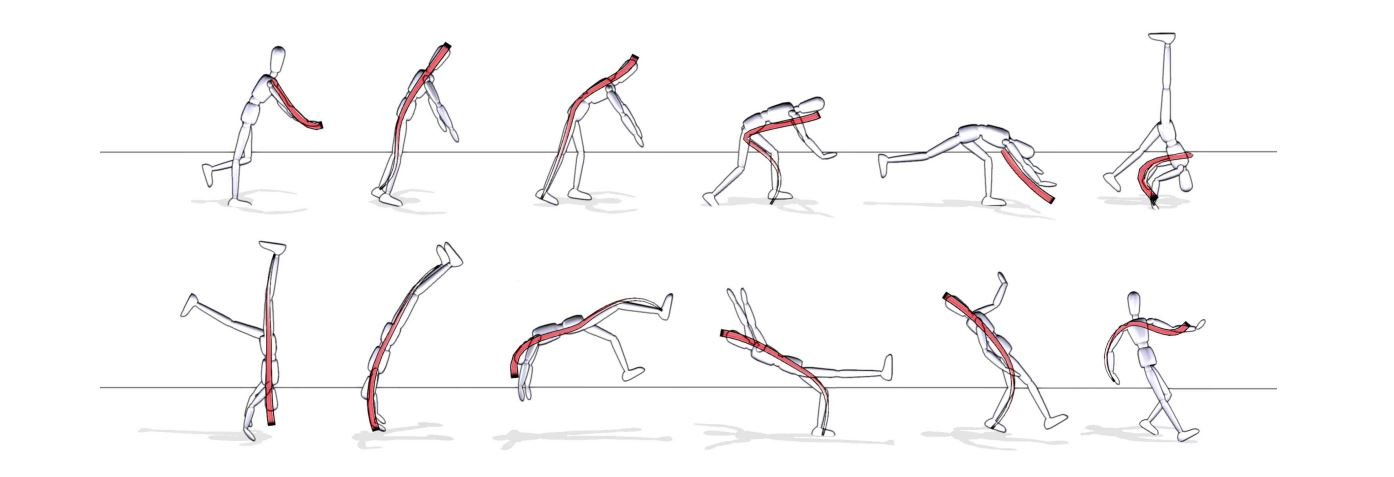
\includegraphics[scale=0.4]{img/baseline}
\caption{One character's keyframes using the line of action technique.}
\end{figure}

The Line of Action: an Intuitive Interface for Expressive Character Posing -- 2013\\
Adding dynamics to sketch-based character animations -- 2015\\
Space-time sketching of character animation -- 2015\\
\\
Artist-oriented 3D character posing from 2D strokes -- 2016\\
people in Switzerland also did the posing \\
Sketch to pose in Pixar's presto animation system -- 2015


\section{Graph Theory}
Finding All the Elementary Cycles in a Directed Graph\\
A New Search Algorithm for Finding the Simple Cycles of a Finite Directed Graph\\
An Algorithm for Combining Graphs Based on Shared Knowledge

\section{Generating Animation}
%\subsection{cleaning/editing animation}
FootSee: an Interactive Animation System\\
Footskate Cleanup for Motion Capture Editing\\
SketchiMo: Sketch-based Motion Editing for Articulated Characters -- 2016\\
sketching for editing trajectories and poses

%\subsection{retargeting motion}
Retargetting Motion to New Characters\\
Using an Intermediate Skeleton and Inverse Kinematics for Motion Retargeting

%\subsection{generating animation}
Motion Graphs\\
Style-Based Inverse Kinematics -- 2004\\
generative models for motion capture sequences used to build animations\\\\
Displacement constraints for interactive modeling and animation of articulated structures -- 1994\\
fitting geometric constraints using physics\\\\
A constrained inverse kinematics technique for real-time motion capture animation -- 1999\\
Dancing-to-Music Character Animation

%\subsection{synthesis}
Synthesizing Dance Performance Using Musical and Motion Features -- 2006\\
between music and an animation generated from a motion graph built from motion capture
